
\begin{problem}
Construct a geometric example showing a compact set $\mathcal{A}$
that does not have a unique best approximation to a point in $\mathds{R}^n$.
\end{problem}
 
\begin{solution}  
\begin{figure}[!ht]
  \centering
  \includegraphics[scale = 0.2]{drawing_task_1.png}
  \label{fig:task_1}
\end{figure}
In figure \ref{fig:task_1} both the point $a^*$ and $a$ are best
approximations. From the theorems concerning uniqueness we see that
it is that the approximation set is {\bf not convex} that is causing the
uniqueness not to be guarantied.
\end{solution}

%%% Local Variables:
%%% TeX-master: "report.tex"
%%% End:
